

\myNewSlide
\section*{Cartoon time courtesy of the \citet{Kim2000} view of tree space}
\begin{picture}(-0,0)(-0,0)
    \put(-10,-90){\makebox(30,-150)[l]{\includegraphics[scale=2.5]{/home/mtholder/Documents/ku_teaching/BIOL-848-2013/images/Kim-treespace.pdf}}}
\end{picture}

\myNewSlide
\section*{Parsimony-informative Pattern Frequency Space}
\begin{picture}(-0,0)(-0,0)
    \put(10,-140){\makebox(30,-150)[l]{\includegraphics[scale=1.]{/home/mtholder/Documents/ku_teaching/BIOL-848-2013/images/simple-treespace.pdf}}}
\end{picture}

\myNewSlide
\section*{Parsimony-informative Pattern Frequency Space}
\begin{picture}(-0,0)(-0,0)
    \put(10,-140){\makebox(30,-150)[l]{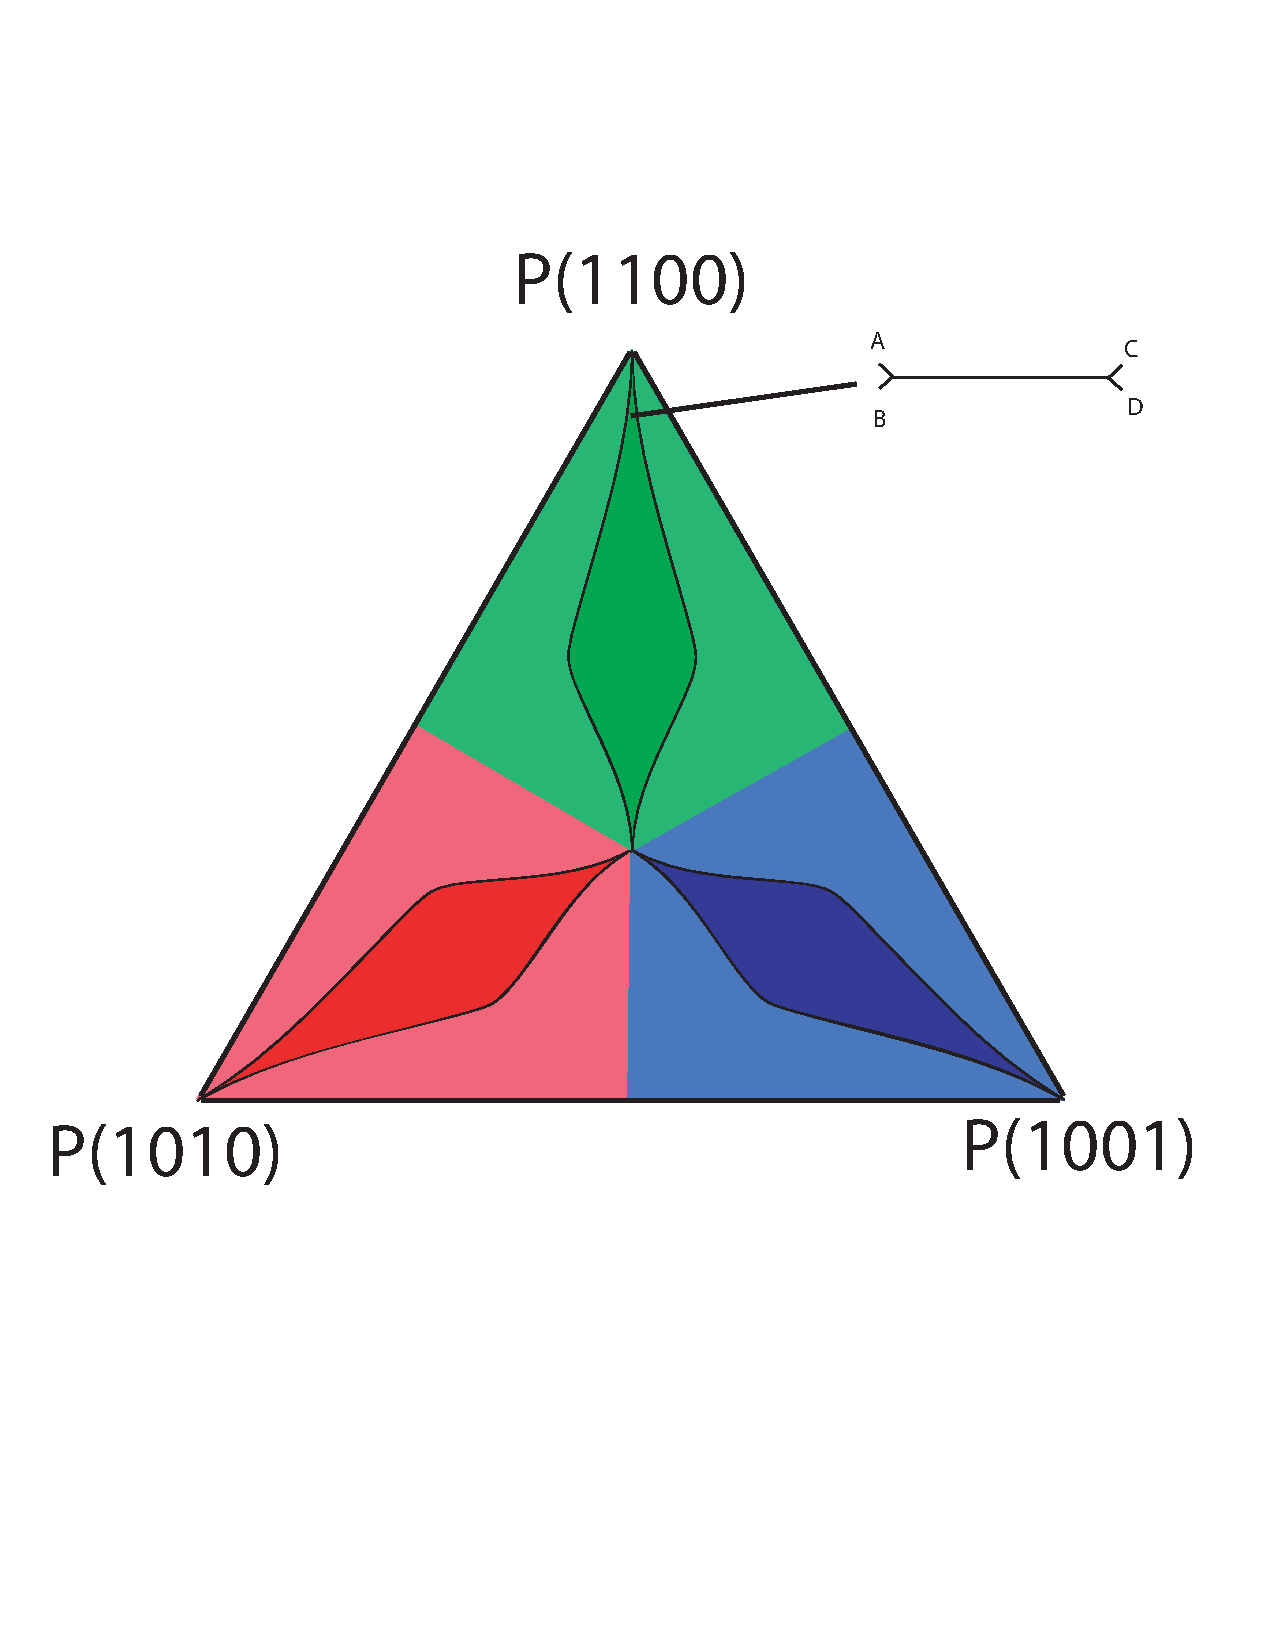
\includegraphics[scale=1.]{../newimages/simple-treespace-clean.pdf}}}
\end{picture}

\myNewSlide
\section*{Parsimony-informative Pattern Frequency Space}
\begin{picture}(-0,0)(-0,0)
    \put(10,-140){\makebox(30,-150)[l]{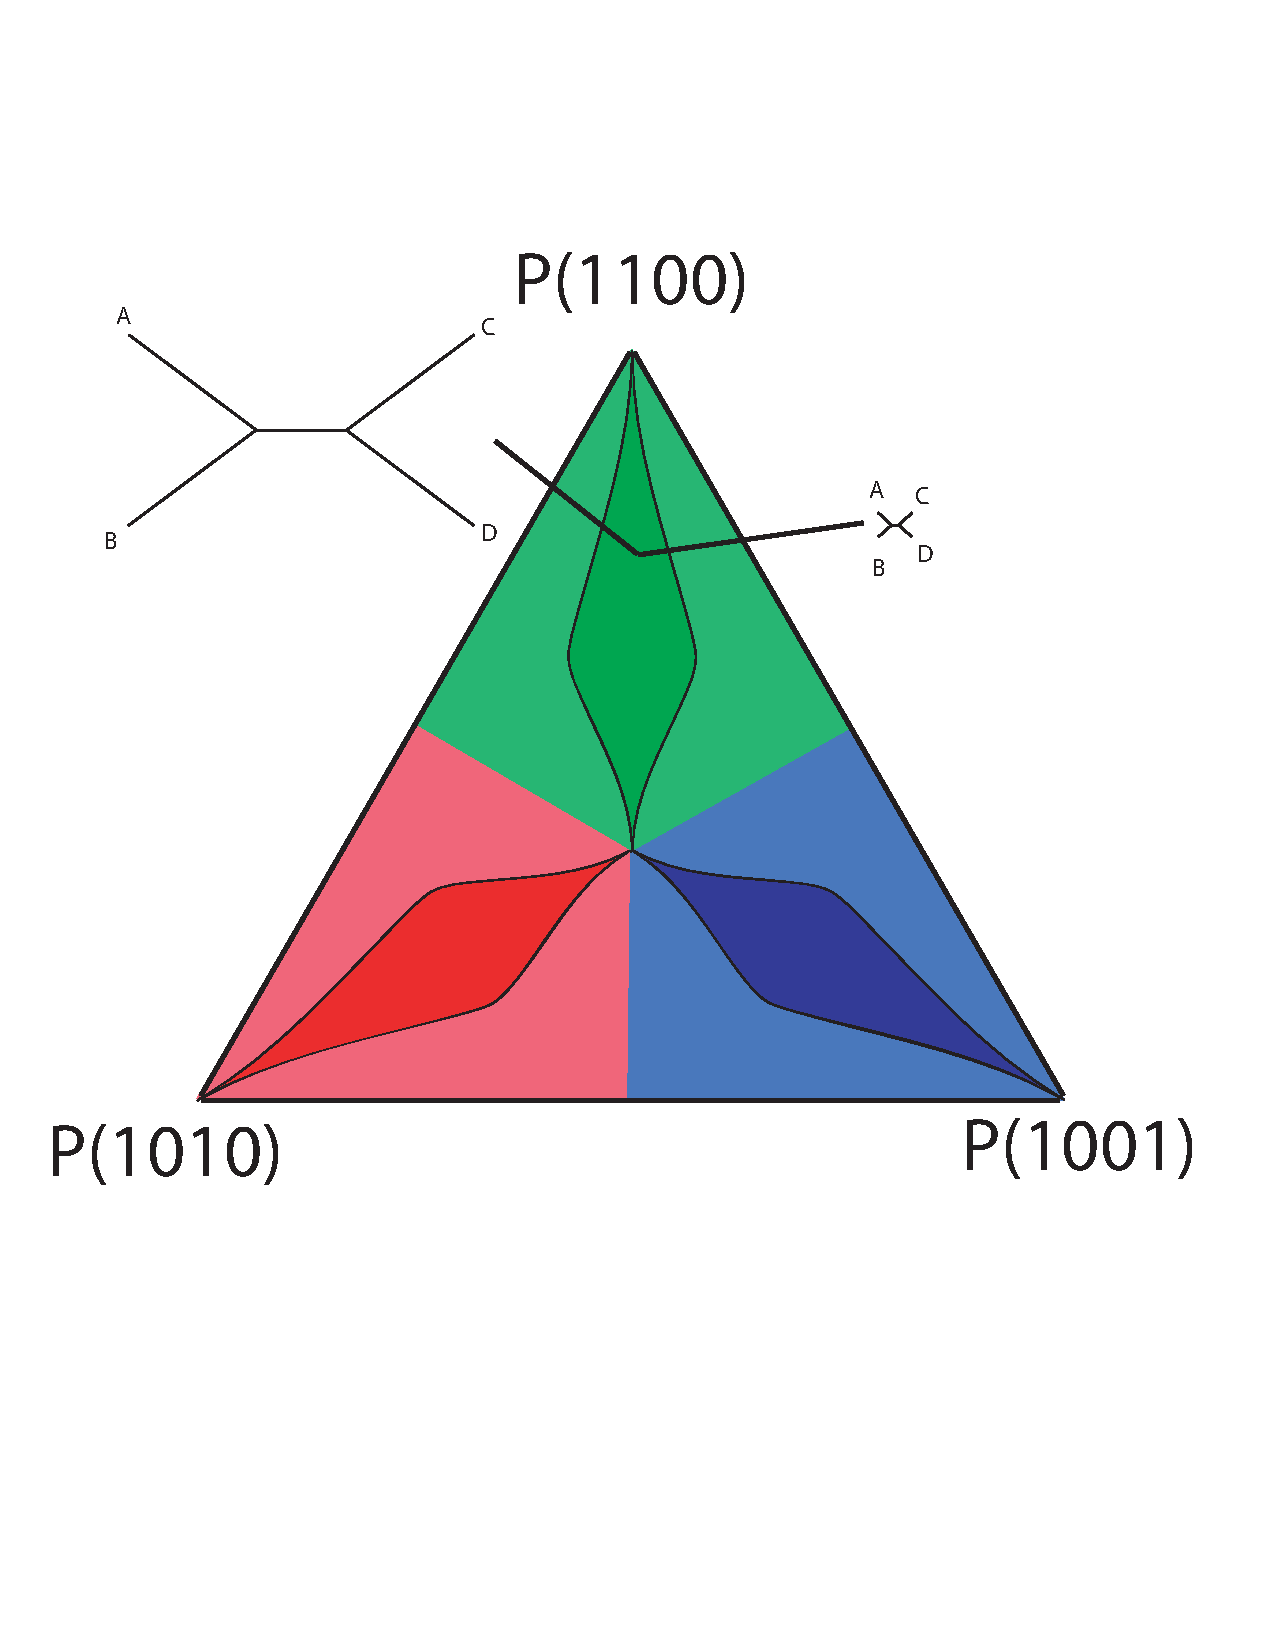
\includegraphics[scale=1.]{../newimages/simple-treespace-messy.pdf}}}
\end{picture}
\myNewSlide
\section*{Parsimony-informative Pattern Frequency Space}
\begin{picture}(-0,0)(-0,0)
    \put(10,-140){\makebox(30,-150)[l]{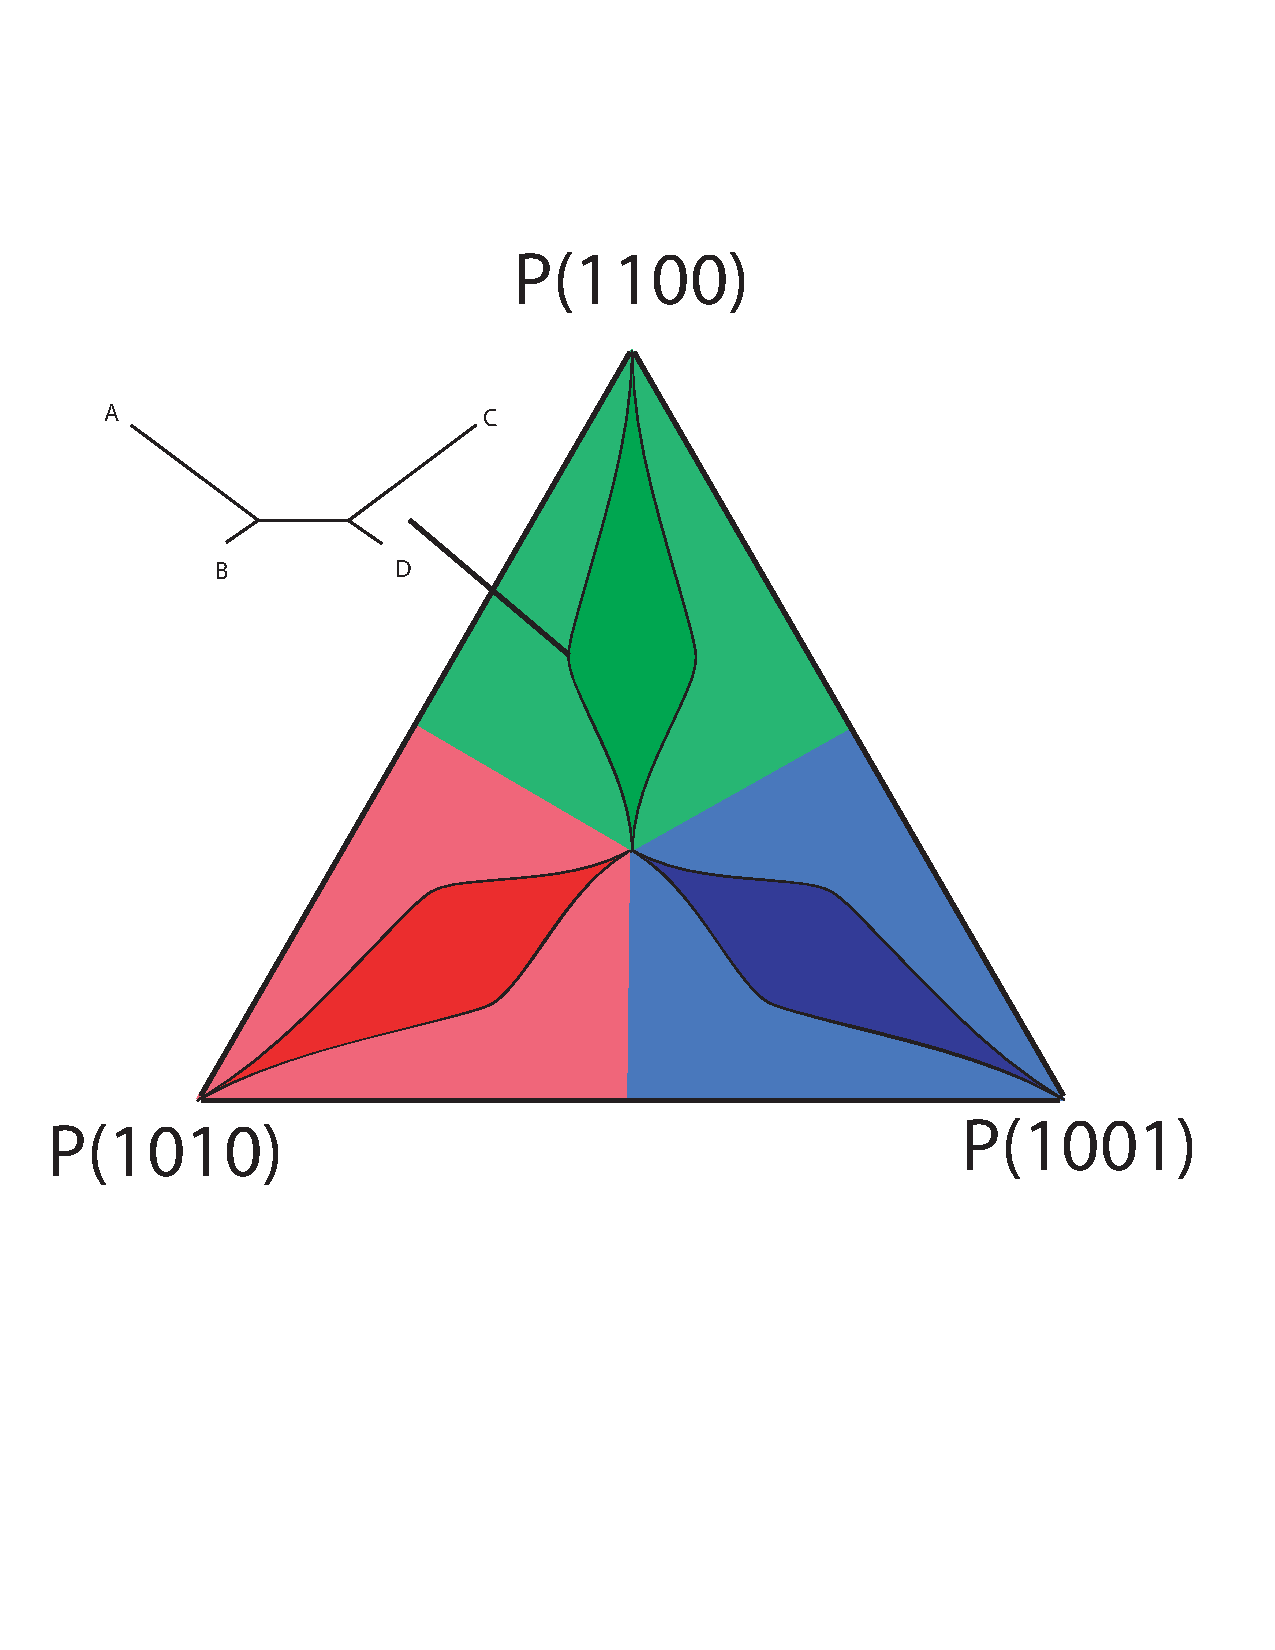
\includegraphics[scale=1.]{../newimages/simple-treespace-lba.pdf}}}
\end{picture}

\myNewSlide
\section*{Pattern Frequency Space With Observed Data}
\begin{picture}(-0,0)(-0,0)
    \put(10,-140){\makebox(30,-150)[l]{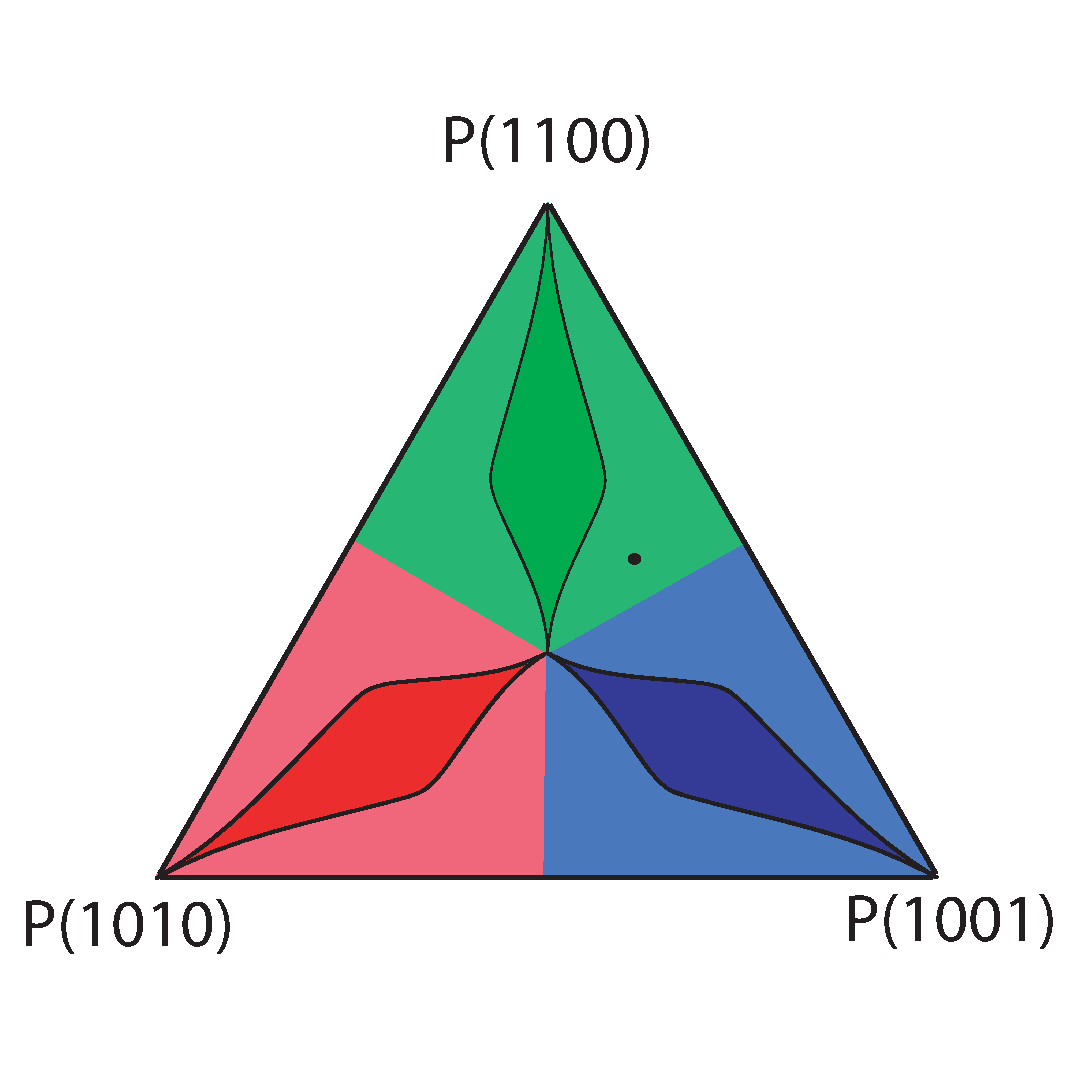
\includegraphics[scale=1.]{../newimages/simple-treespace-sample.pdf}}}
    \put(370,-183){$f_X$}
\end{picture}


\myNewSlide
\section*{ML scores in Pattern Frequency Space}
\begin{picture}(-0,0)(-0,0)
    \put(10,-120){\makebox(30,-190)[l]{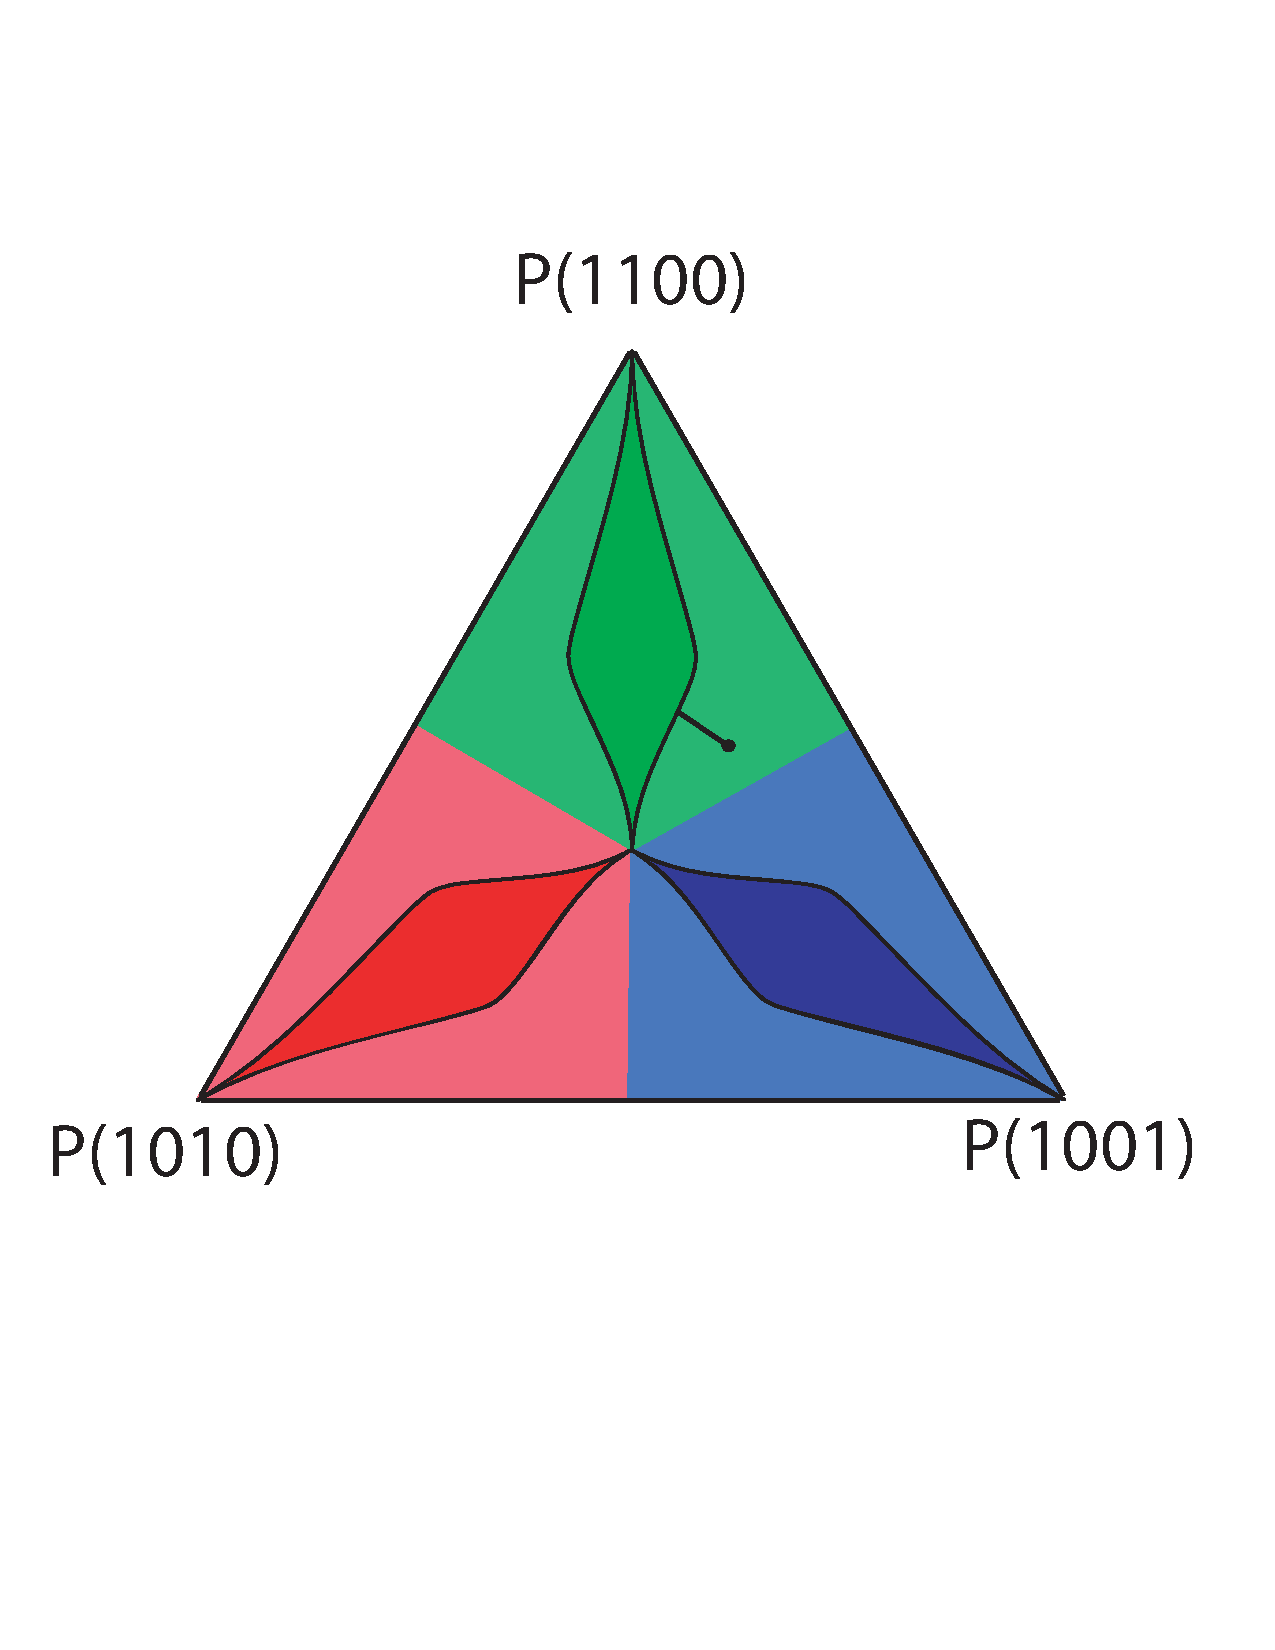
\includegraphics[scale=1.]{../newimages/simple-treespace-pp1v2.pdf}}}
    \put(-30,-0){$\ln L(T_1 \mid X) = -D_{KL}(f_X \mid f_{T_1})$}
\end{picture}

\myNewSlide
\section*{LR statistics in Pattern Frequency Space}
\begin{picture}(-0,0)(-0,0)
    \put(10,-120){\makebox(30,-190)[l]{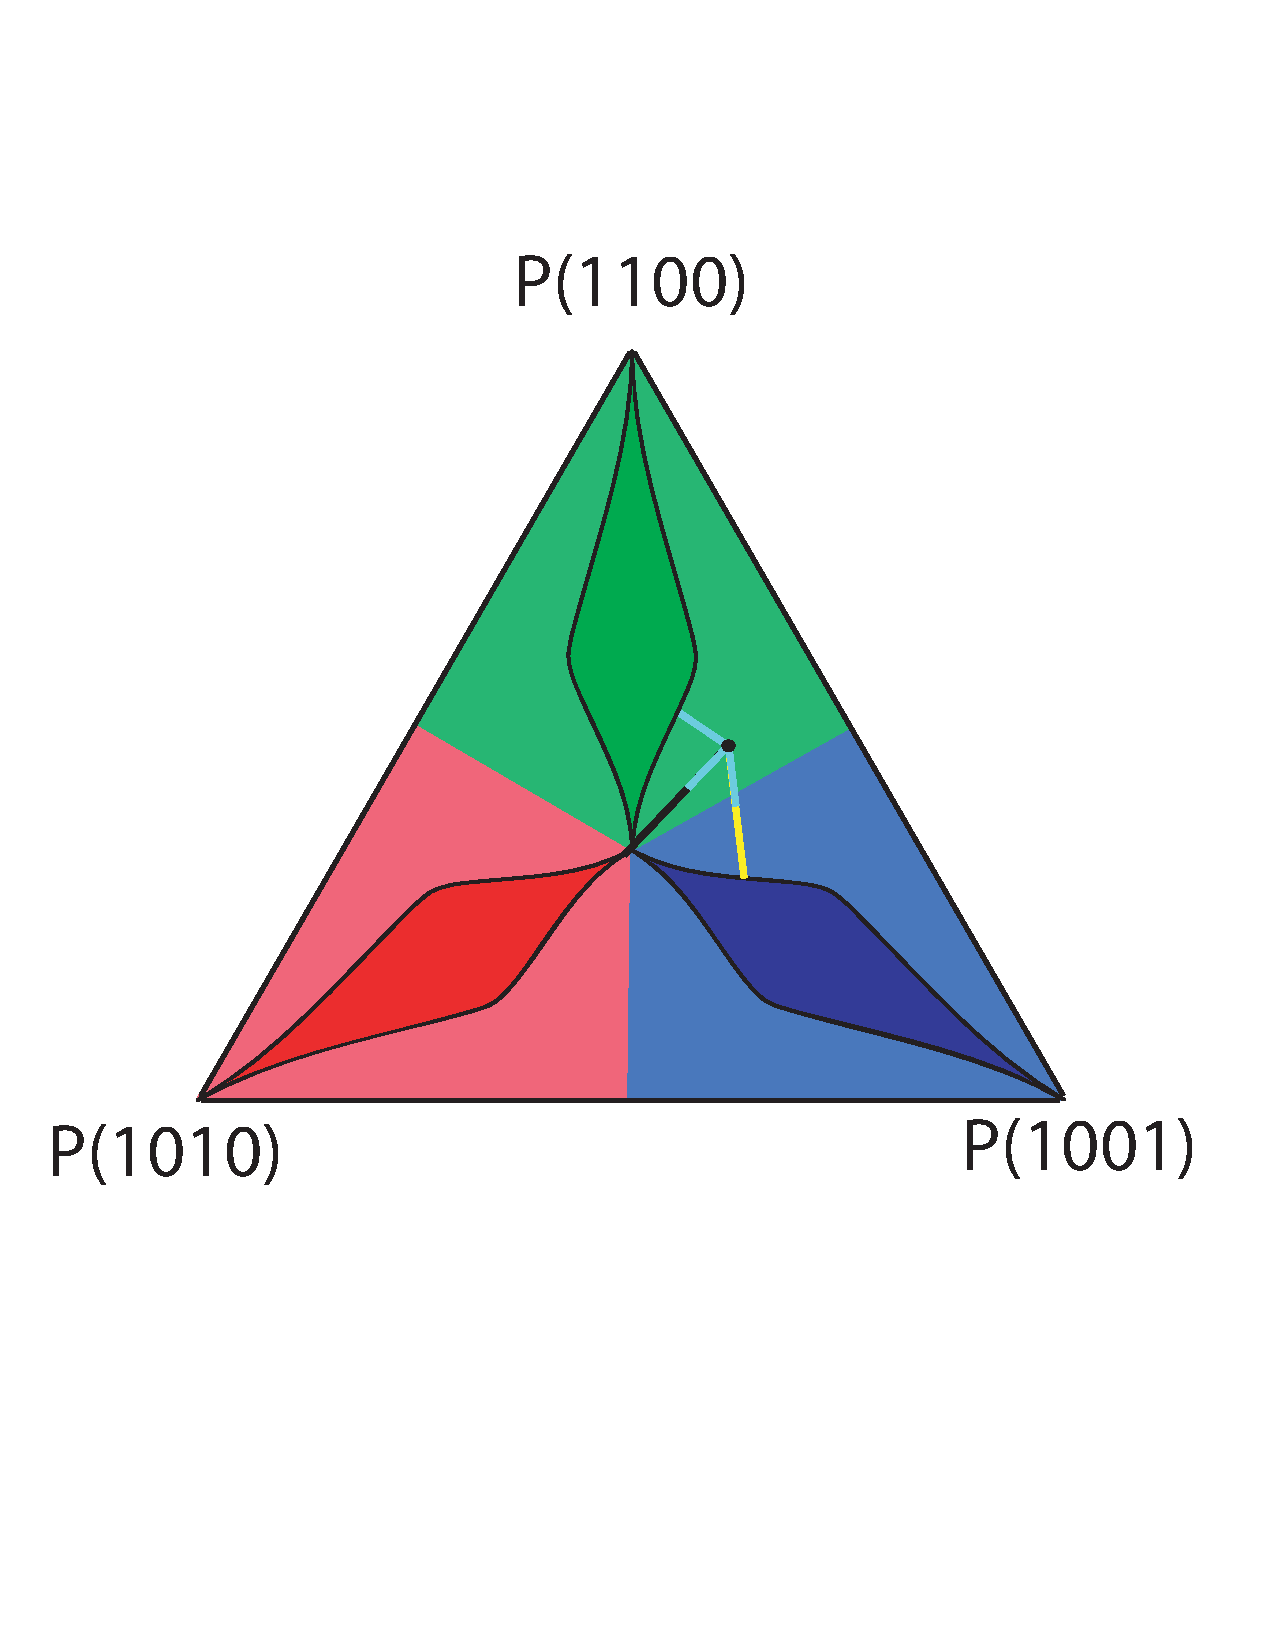
\includegraphics[scale=1.]{../newimages/simple-treespace-ppv2.pdf}}}
    \put(-50,-0){Black is $\ln L(T_{AB}) - \ln L(T_{AC})$}
    \put(370,-0){Yellow is $\ln L(T_{AB}) - \ln L(T_{AD})$}
    
\end{picture}


\myNewSlide
\section*{KH Test in Pattern Frequency Space}
\begin{picture}(-0,0)(-0,0)
    \put(10,-120){\makebox(30,-190)[l]{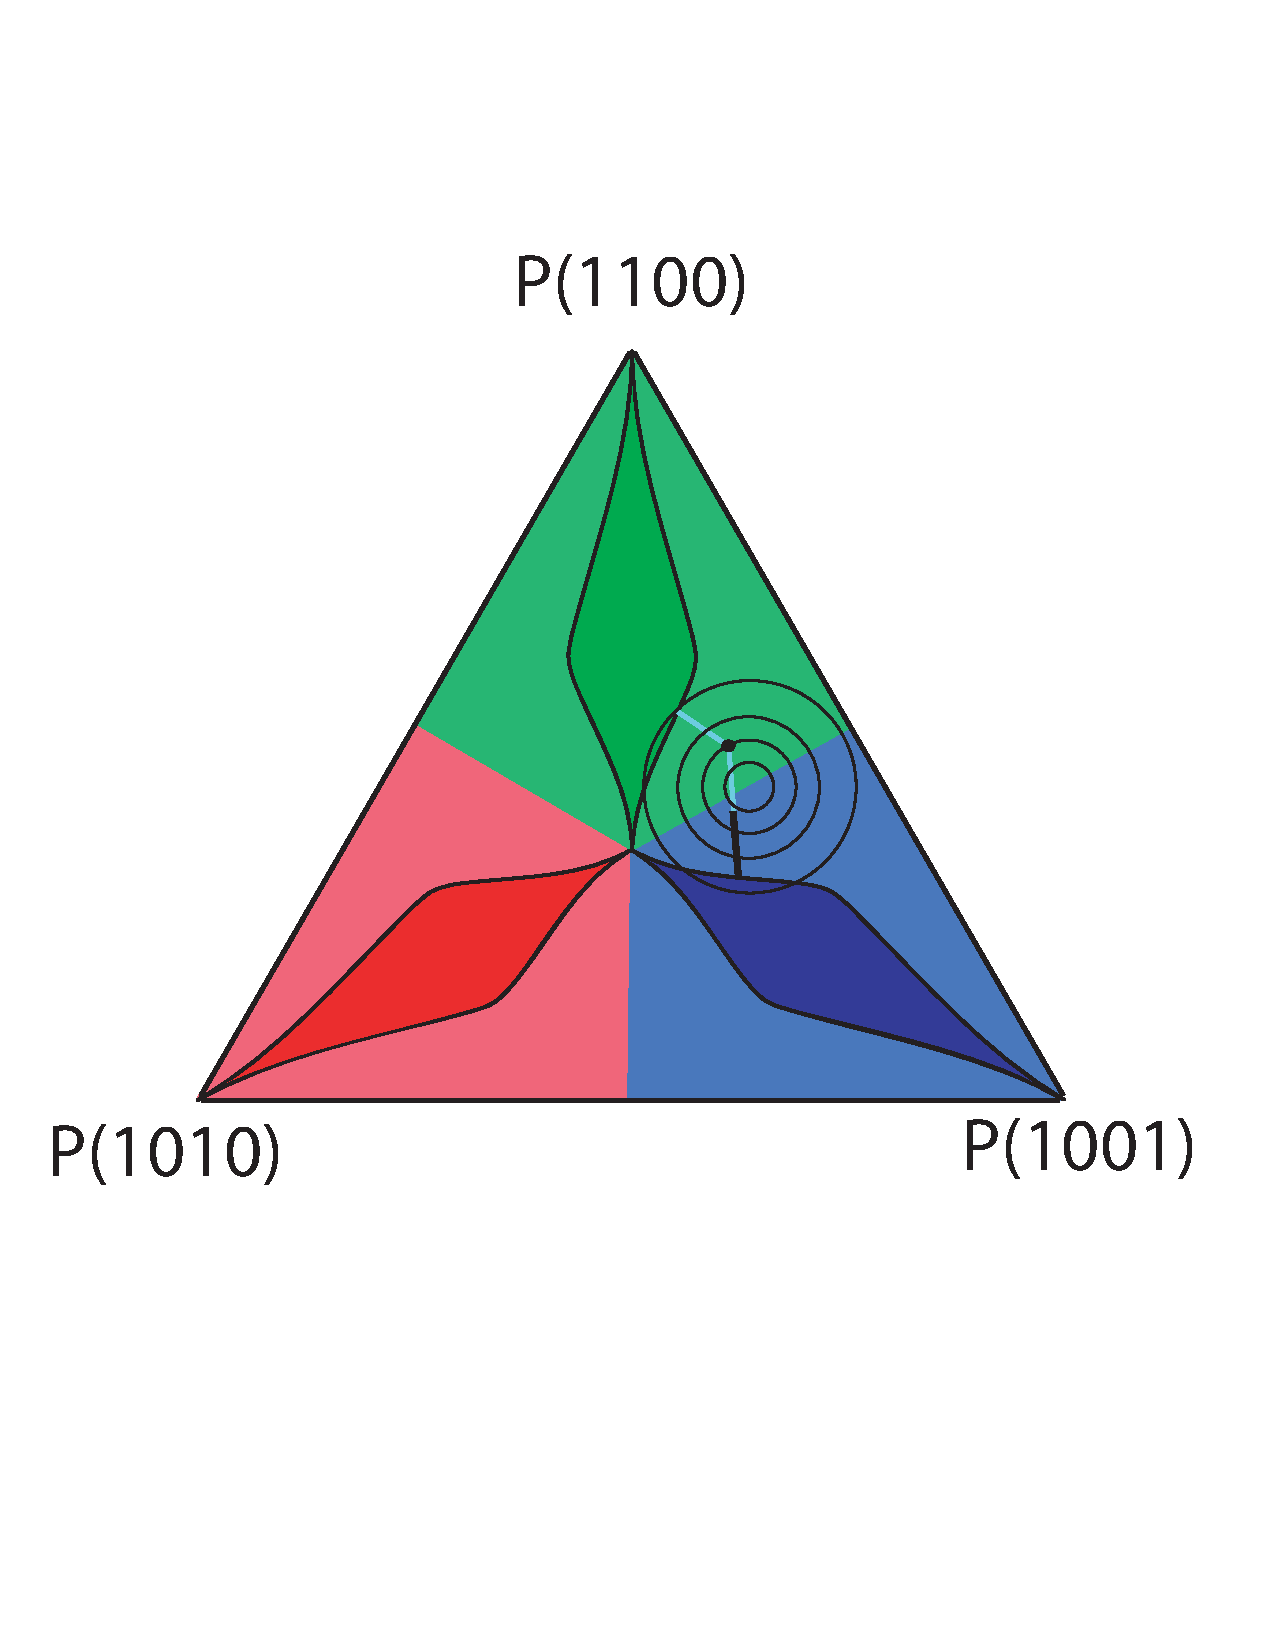
\includegraphics[scale=1.]{../newimages/simple-treespace-kh.pdf}}}
    \put(-50,-0){Uses the $\delta$ test statistic}
    \put(-40,-30){and a null distribution}
    \put(-40,-60){{\em centered} on the boundary}
\end{picture}


\myNewSlide
\section*{Parametric bootstrapping in Pattern Frequency Space}
\begin{picture}(-0,0)(-0,0)
    \put(10,-120){\makebox(30,-190)[l]{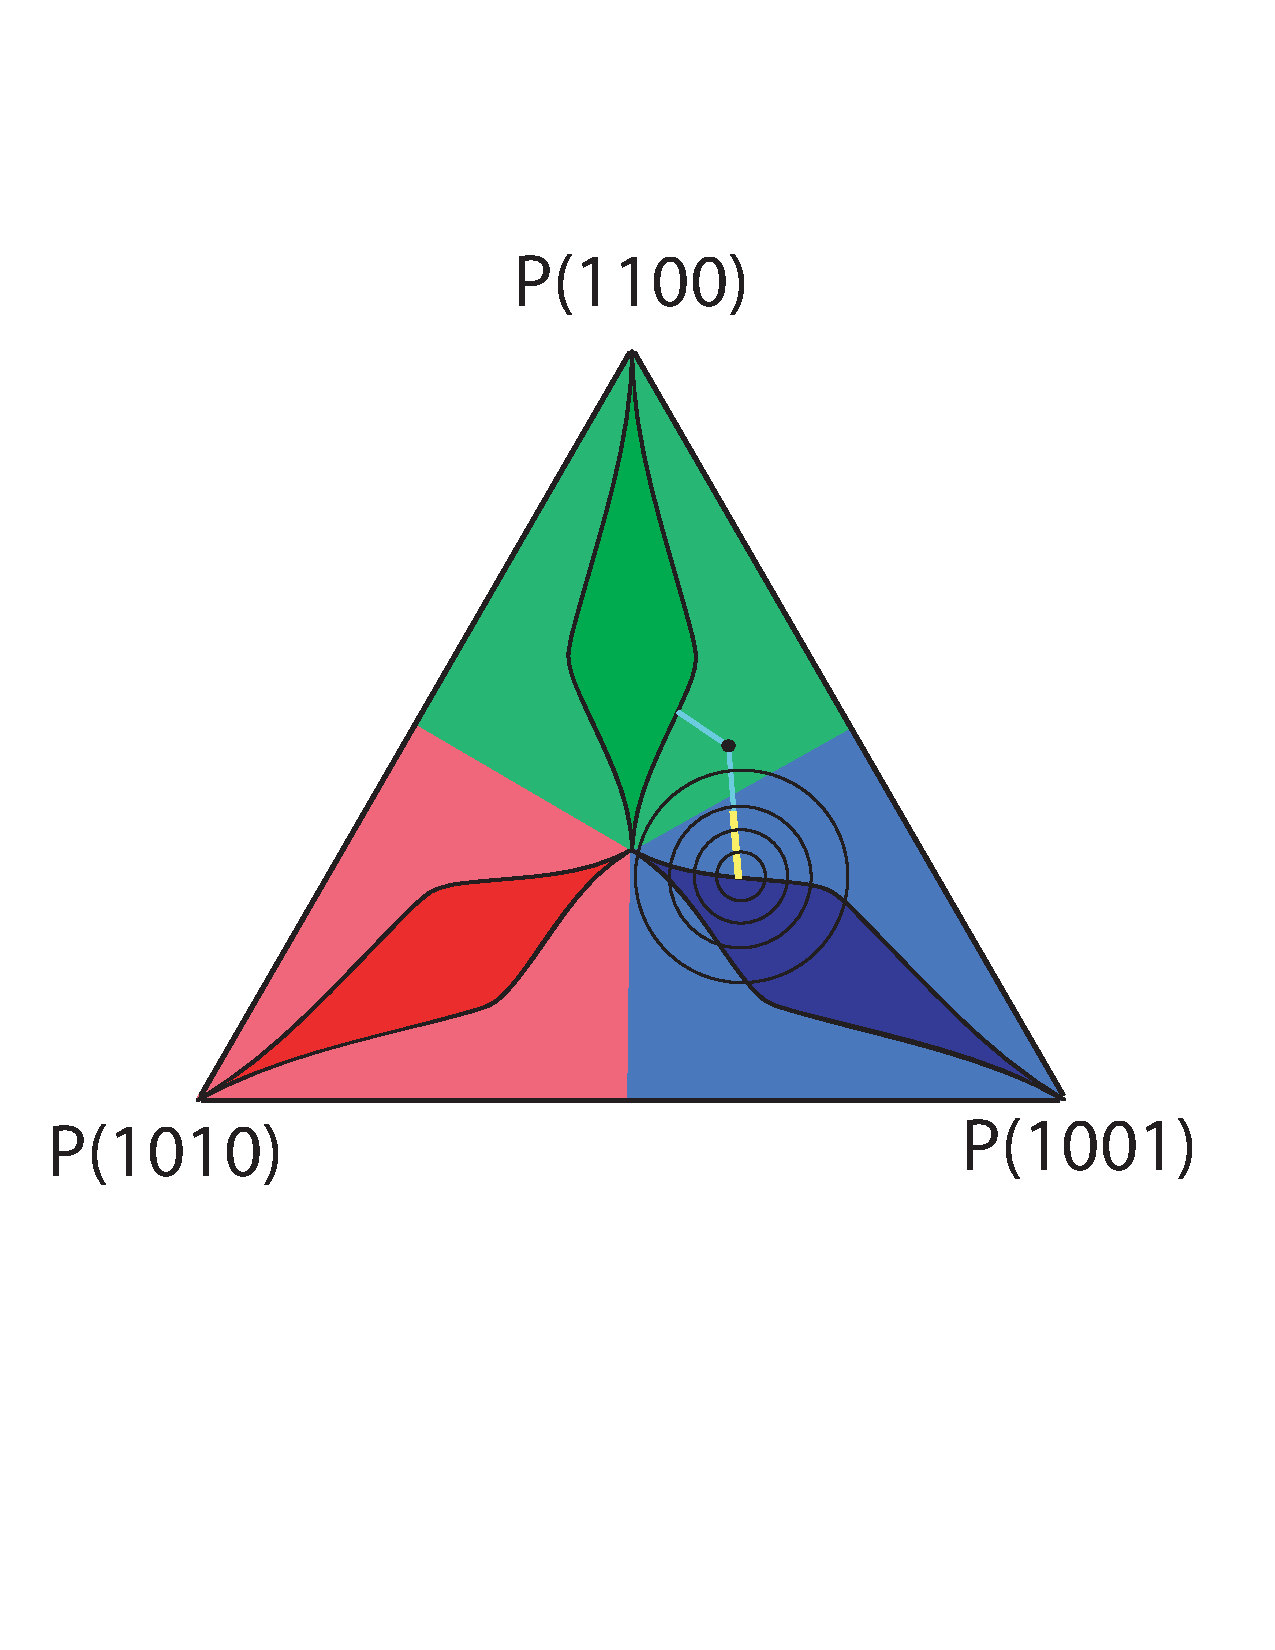
\includegraphics[scale=1.]{../newimages/simple-treespace-parametricBP.pdf}}}
    \put(-50,-0){Uses the $\delta$ test statistic}
    \put(-40,-30){and a null distribution}
    \put(-40,-60){{\em centered} on point that}
    \put(-40,-90){arises from the best}
    \put(-40,-120){tree in $H_0$}
\end{picture}
\myNewSlide

\begin{picture}(-0,0)(-0,20)
    \put(10,-120){\makebox(30,-190)[l]{\includegraphics[scale=1.]{../newimages/simple-treespace-susko-parametricBoot2.pdf}}}
    \put(-50,60){Susko modification to}
    \put(-50,30){param. boot.:}
    \put(-50,-0){Uses the $\delta$ test statistic}
    \put(-40,-30){and a null distribution}
    \put(-40,-60){{\em centered} on point that}
    \put(-40,-90){arises from the best}
    \put(-40,-120){tree in $H_0$ but with }
    \put(-40,-150){branches in conflict}
    \put(-40,-180){with $\hat{T}$ constrained.}
    \put(-40,-210){to be 0.}
\end{picture}

\myNewSlide
\section*{\citet{EfronHH1996} view of tree space}
\begin{picture}(-0,0)(-0,0)
    \put(-10,-90){\makebox(30,-150)[l]{\includegraphics[scale=3]{/home/mtholder/Documents/ku_teaching/BIOL-848-2013/images/EfronHH-treespace-fig.pdf}}}
\end{picture}

\myNewSlide
\section*{Parsimony-informative Pattern Frequency Space}
\begin{picture}(-0,0)(-0,0)
    \put(10,-140){\makebox(30,-150)[l]{\includegraphics[scale=1.]{/home/mtholder/Documents/ku_teaching/BIOL-848-2013/images/simple-treespace.pdf}}}
\end{picture}
 
\myNewSlide
\begin{picture}(-0,0)(-0,0)
    \put(20,0){\normalsize Imagine hypothesis tests of locations with different border shapes:}
    \put(-10,-90){\makebox(30,-150)[l]{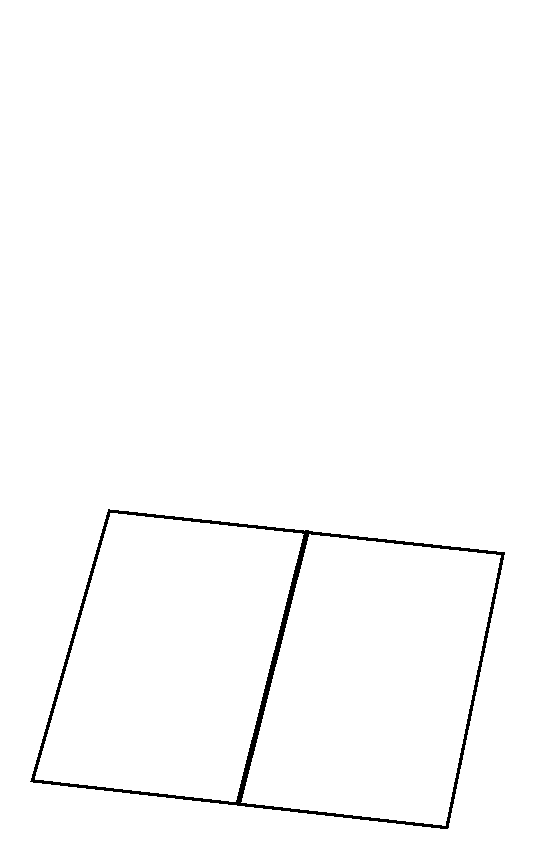
\includegraphics[scale=1.2]{../newimages/boundarylandscape.pdf}}}
    \put(300,-90){\makebox(30,-150)[l]{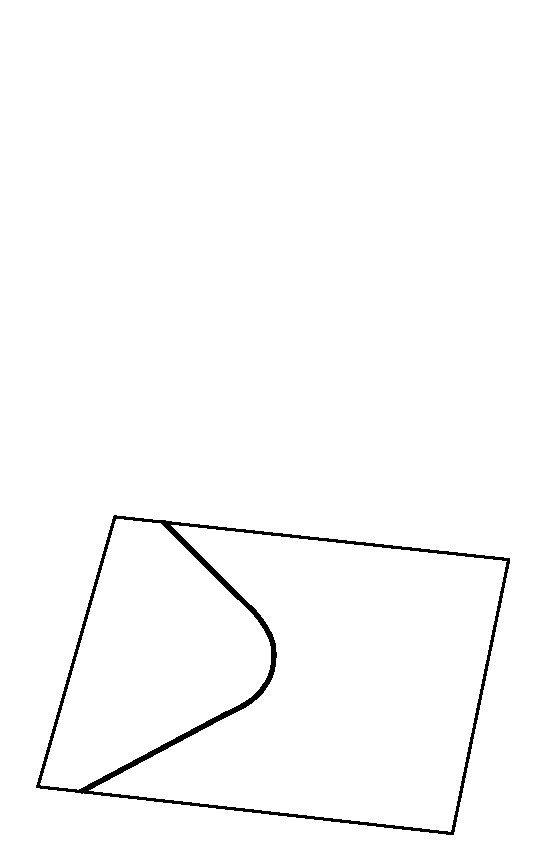
\includegraphics[scale=1.2]{../newimages/curved_boundarylandscape.pdf}}}
    \put(80,-290){$H_0$}
    \put(160,-330){$H_1$}
    \put(380,-290){$H_0$}
    \put(490,-330){$H_1$}
\end{picture}

\myNewSlide
\begin{picture}(-0,0)(-0,0)
    \put(40,0){\large Similar dataset with point estimates (red dot) in $H_1$}
    \put(20,-40){\large Green dot is the hardest set of locations in $H_0$ to reject.}
    \put(-10,-90){\makebox(30,-150)[l]{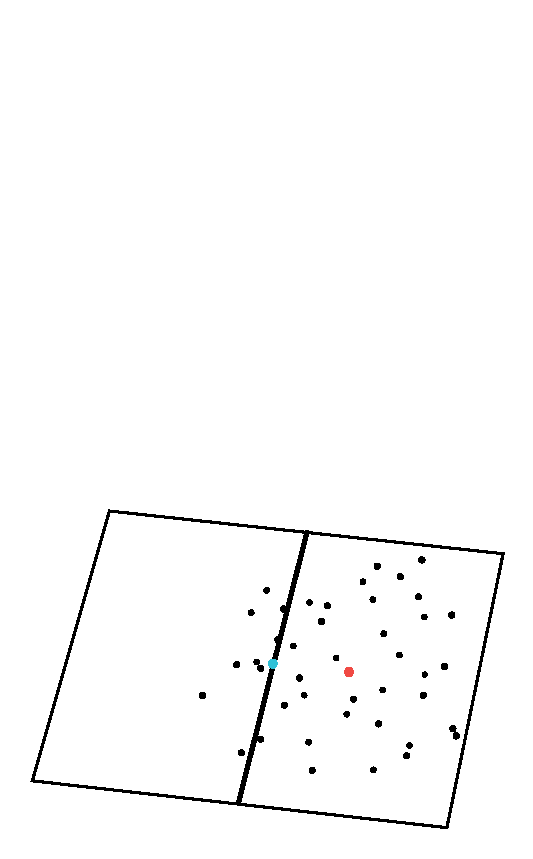
\includegraphics[scale=1.2]{../newimages/boundarylandscape_pts.pdf}}}
    \put(300,-90){\makebox(30,-150)[l]{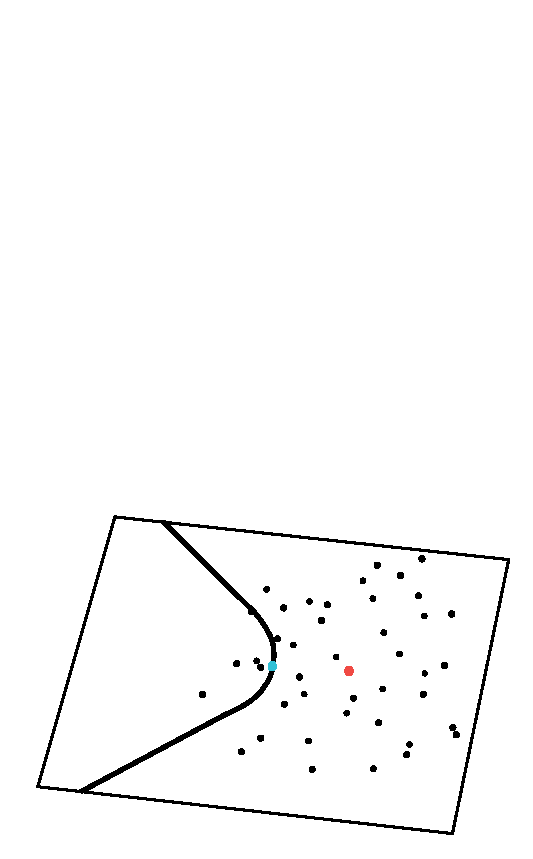
\includegraphics[scale=1.2]{../newimages/curved_boundarylandscape_pts.pdf}}}
\end{picture}



\myNewSlide
\section*{Non-parametric Bootstrapping in Pattern Frequency Space}
\begin{picture}(-0,0)(-0,0)
    \put(10,-150){\makebox(30,-150)[l]{\includegraphics[scale=1.]{/home/mtholder/Documents/ku_teaching/BIOL-848-2013/images/simple-treespace-boot.pdf}}}
\end{picture}

\myNewSlide
\section*{Bootstrapping in Pattern Frequency Space (if you had more data)}
\begin{picture}(-0,0)(-0,0)
    \put(-50,-0){AU Test uses multiple sequence}
    \put(-40,-30){lengths to correct BP for}
    \put(-40,-60){any curvature in the  }
    \put(-40,-90){boundary between}
    \put(-40,-120){trees}
    \put(10,-150){\makebox(30,-150)[l]{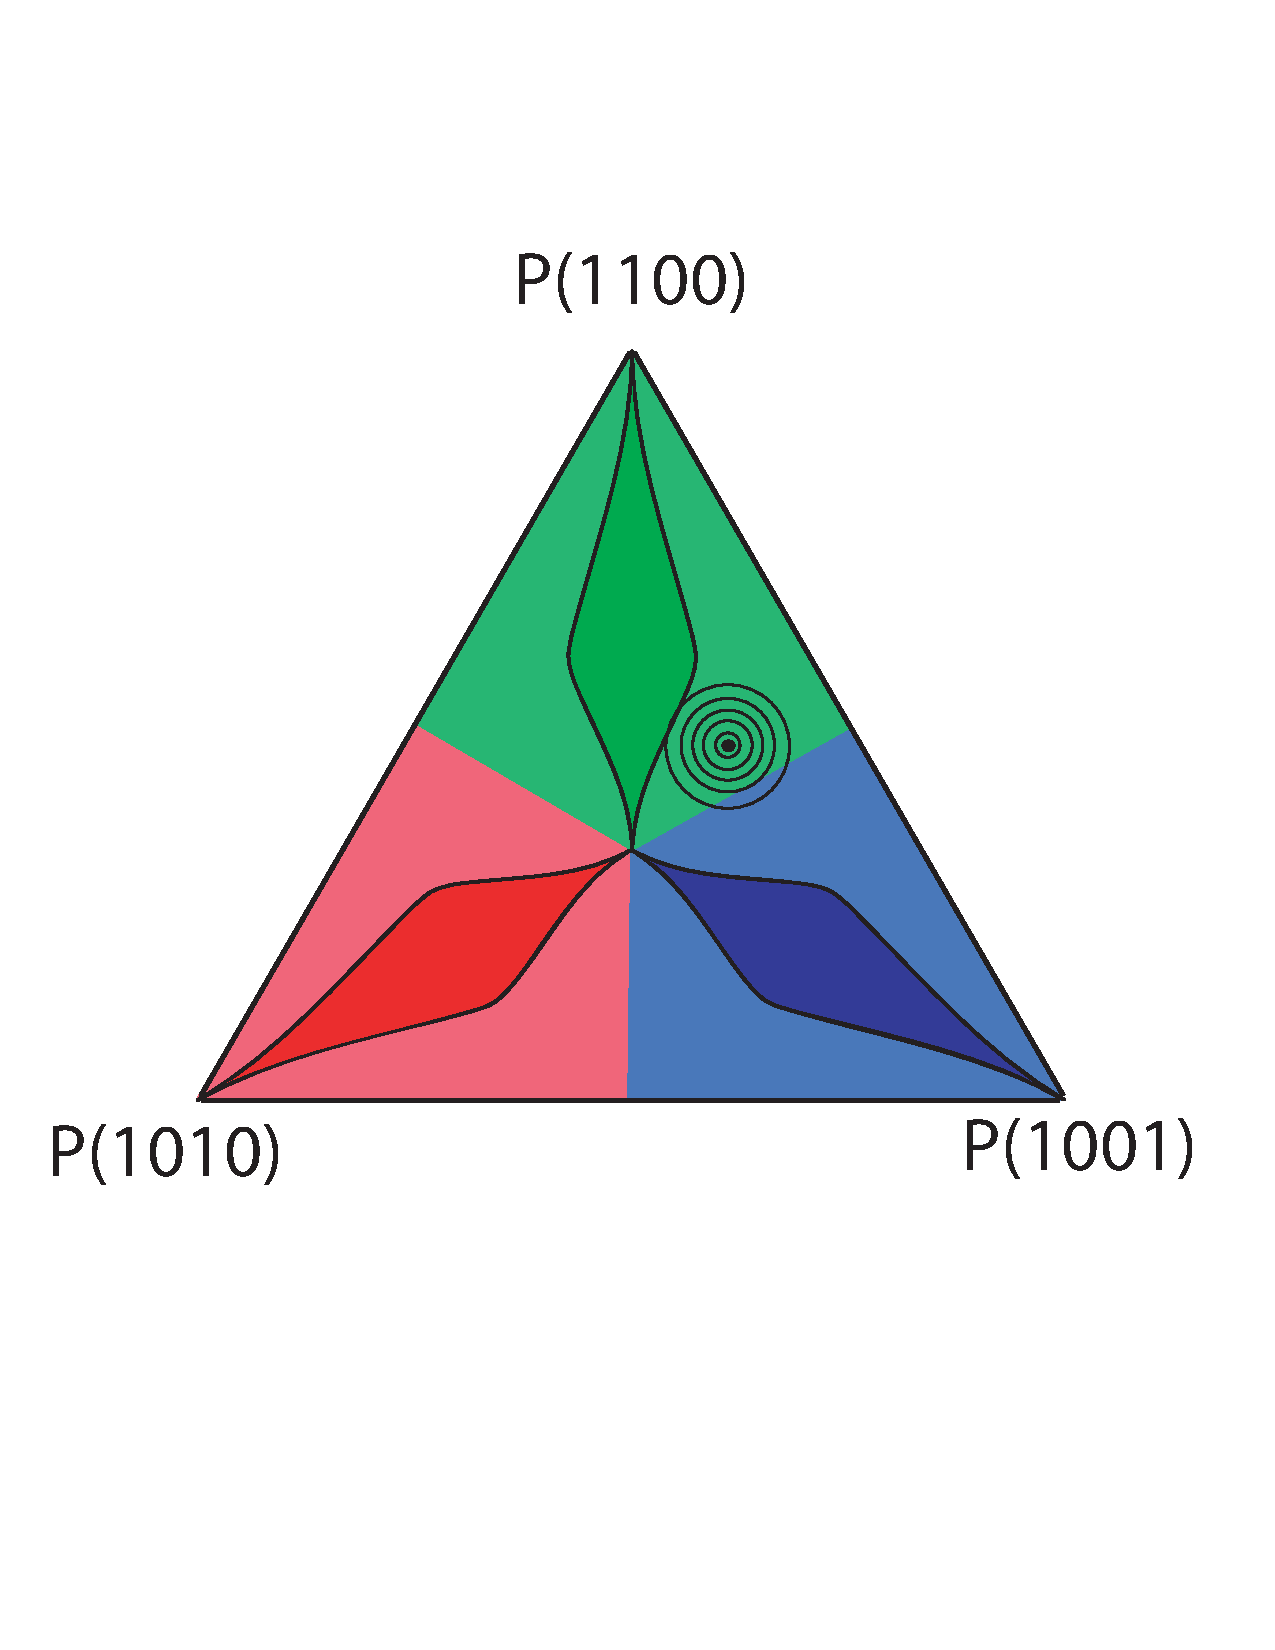
\includegraphics[scale=1.]{../newimages/simple-treespace-boot-more.pdf}}}
\end{picture}



\myNewSlide
\section*{aBP in Pattern Frequency Space}
\begin{picture}(-0,0)(-0,0)
    \put(-50,-0){Null distribution for BP}
    \put(-40,-30){is calculated using}
    \put(-40,-60){Normal approximations from}
    \put(-40,-90){polytomy}
    \put(10,-150){\makebox(30,-150)[l]{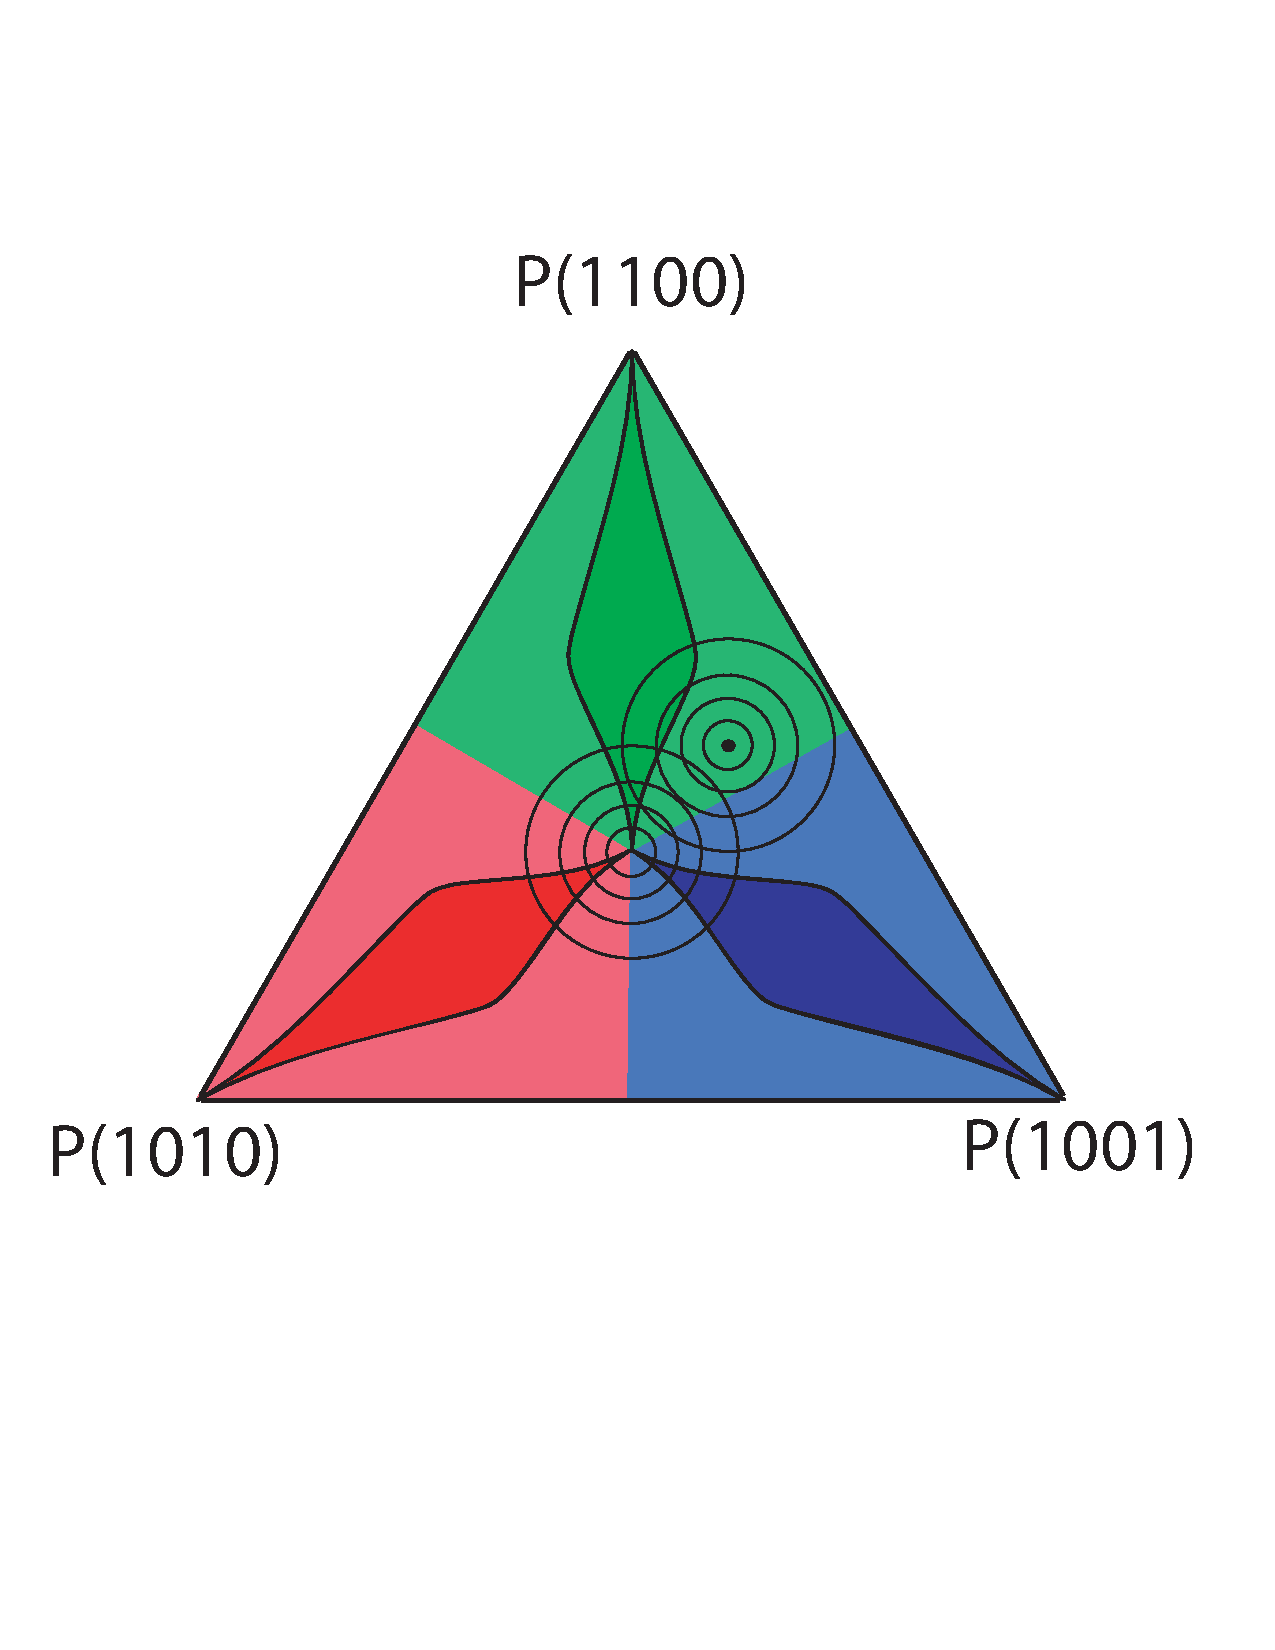
\includegraphics[scale=1.]{../newimages/simple-treespace-abp.pdf}}}
\end{picture}

\myNewSlide
\section*{aLRT and aBayes in Pattern Frequency Space}
\begin{picture}(-0,0)(-0,0)
    \put(10,-120){\makebox(30,-190)[l]{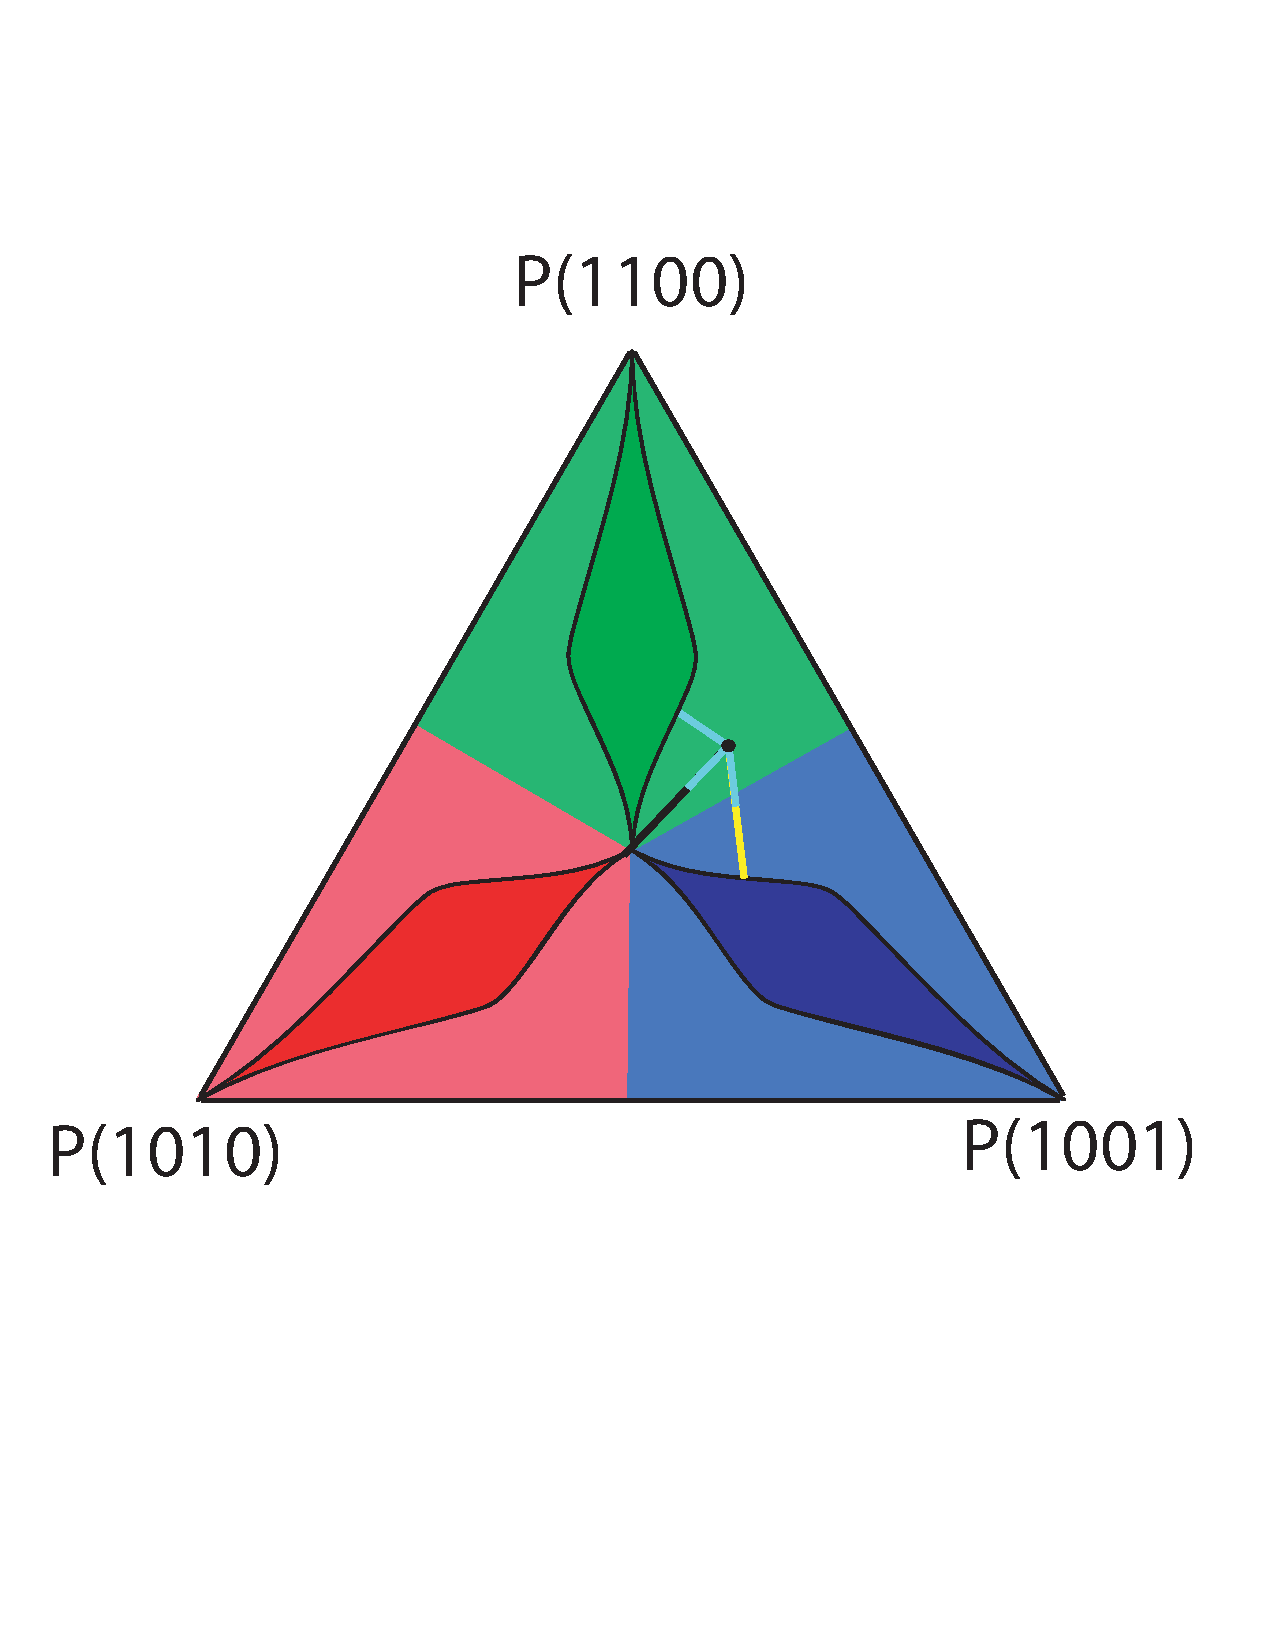
\includegraphics[scale=1.]{../newimages/simple-treespace-ppv2.pdf}}}
    \put(-50,-0){In aLRT, we use mixtures of $\chi^2$}
    \put(-40,-30){and selection bias corrections}
    \put(-40,-60){to calculate the $P$-value.}
    \put(370,-0){In aBayes, we normalize}
    \put(380,-30){the ML scores to sum to 1}
\end{picture}



